\documentclass[11pt]{article}

\usepackage[margin=1in]{geometry}
\usepackage{graphicx}
\usepackage{booktabs}
\usepackage{amsmath}
\usepackage{amssymb}
\usepackage{caption}
\usepackage[hidelinks]{hyperref}
\usepackage{times}
\usepackage{longtable}
\usepackage{adjustbox}
\usepackage{microtype}

\setlength{\parindent}{0pt}
\setlength{\parskip}{0.72em}
\captionsetup{font=small,labelfont=bf,skip=4pt}
\renewcommand{\arraystretch}{1.08}
\setlength{\emergencystretch}{2em}

\title{\vspace{-2em}A Dynamic Orchestrator under a Forced Compute Ladder:\\
Off-the-shelf Agent Harnesses against the Fixed Rule}
\author{Study \texttt{openrouter\_dynorch\_v1} (ladder: \texttt{openrouter\_forced\_budget\_v2})}
\date{\today}

\begin{document}
\maketitle
\vspace{-1.5em}

\section*{Abstract}

The forced-budget ladder found that, at equal generated tokens $C = kA$, one deep call beats every structured
multi-call allocation: deep/16 delivers 0.792 macro accuracy against 0.417 for
sample/16 and an oracle pass@16 of 0.580. This study asks whether a dynamic orchestrator beats
that fixed rule: an off-the-shelf agent harness that decides for itself whether to spawn sub-agents, revise or
synthesise, using the same model (Qwen3.8-27B) under the same total completion budget. Two harnesses,
OpenClaude 0.13.0 (H1) and Codex CLI 0.156.1 (H3), and a harness-free control (H0) ran on the
ladder's 96 items at rungs $C/A \in \{1, 2, 4, 8, 16, 25\}$. A metering proxy caps every call at the
remaining budget and grants one grace of at most 1,024 tokens outside $C$, as the ladder's
uncounted answer call did.

The harnesses did not orchestrate. No harness run spawned a sub-agent: 0 of the 1,152
harness runs in the core, and 0 of all 1,296 harness runs across canary, pilot,
main and reruns. OpenClaude made exactly one model call in each of its 576 runs; Codex
made a second call in 12 of 576 runs, each time after
a planning call, never a delegation.

At $C = 16A$ H1 delivers 0.667 [0.573, 0.760], H3
0.646 [0.552, 0.729], and the same-week, same-host control H0
0.719. In the pre-registered primary family (Holm over four, macro, 96 paired items),
H1/16 $-$ deep/16 = $-$12.5 points [$-$21.3,
$-$5.2] and H3/16 $-$ deep/16 = $-$14.6 points
[$-$23.4, $-$7.1]. The frozen reading rule gives the
same verdict for both harnesses: dynamic orchestration loses to the fixed rule. Both are above the sampling baseline:
H1/16 $-$ sample/16 = +25.0 and H3/16 $-$ sample/16 =
+22.9 points.

The shortfall against deep/16 is not evidence against orchestration, because none took place. The harnesses' one
call stops on its own at about 0.59 of the cap at $16A$, while the ladder forced
deep/16 to spend all 16,384 tokens. Per realized token, the harness cells lie on or near the deep-call curve.

\section{Design}

\subsection{Arms, cells and budget}

Figure~\ref{fig:design} shows the cells. Every run of every arm is served by the same metering proxy against the
same pinned model, template and sampling as the ladder. The budget unit is completion tokens (reasoning and
visible text of every call the proxy serves under the run's key, sub-agents included); the harness is told its
budget in one sentence of the task prompt and receives HTTP 402 once it is exhausted. Calls of one run are served
one at a time, each granted $\max\_tokens = C - \text{spent}$, so the cap is exact by construction: no run in this
report exceeded its cap (0 cap overruns among 1,728 runs). A root call that
hits its grant mid-reasoning is closed with one answer continuation of at most 1,024 tokens outside $C$
(``grace''), mirroring the ladder's answer call, which was also outside $C$.

\begin{figure}[htbp]
\centering
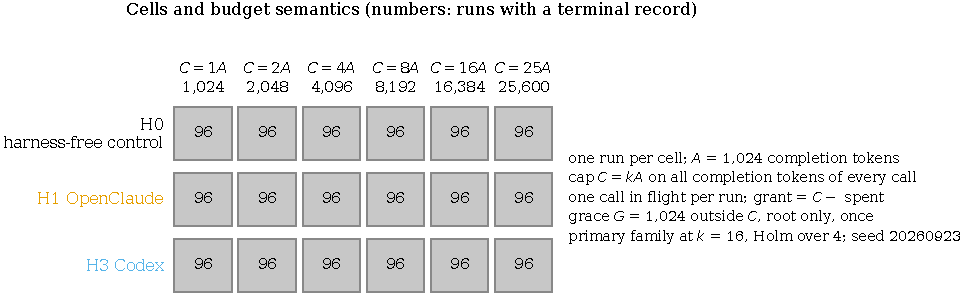
\includegraphics[width=\textwidth]{figures/d1_design.pdf}
\caption{Cells of the core (numbers: runs with a terminal record per arm and rung) and the budget semantics
every arm shares.}
\label{fig:design}
\end{figure}

\subsection{Comparison frames}

F1 (primary) pairs each harness cell at nominal cap $C$ with the ladder configurations at $C = B\cdot R\cdot A$.
The ladder's $C$ counted reasoning only, so F1 is conservative against the harness by one uncounted answer per
ladder call: on average 302 tokens for deep/16 and
5,338 for sample/16. F2 (descriptive) puts both sides at realized total
completion tokens; the dollar frontier uses charged USD and the standardized uncached price.

\subsection{Population and statistics}

Every interval is a paired, item-clustered bootstrap over the fixed population of 96 main items
(10,000 replicates, seed 20260923), one population per contrast, items kept together
across columns. A row exists for every planned cell before a run starts, so no item is ever dropped by the
population builder; 0 cells fall below 95.0\% completeness. The ladder's own point estimates
are reproduced from the merged frame (deep/16 = 0.792 against the sealed
0.792; sample/16 = 0.417 against
0.417); the ladder's intervals are re-drawn per contrast and differ slightly from
the sealed report's joint-population intervals.

\section{Results}

\subsection{Headline at $C = 16A$}

\begin{table}[htbp]
\centering\small
\adjustbox{max width=\textwidth}{\begin{tabular}{lrrrrrrrrr}
\toprule
Benchmark & pass@1 & vote@16 & oracle@16 & private/16 & best non-deep & deep/16 & H0/16 & H1/16 & H3/16 \\
\midrule
AIME 25+26 & 0.333 & 0.375 & 0.465 & 0.500 & 0.500 & 0.833 & 0.792 & 0.792 & 0.875 \\
HMMT Feb 25+26 & 0.217 & 0.208 & 0.302 & 0.292 & 0.292 & 0.792 & 0.750 & 0.667 & 0.583 \\
Omni-MATH $\geq$7 & 0.167 & 0.292 & 0.553 & 0.391 & 0.391 & 0.625 & 0.500 & 0.458 & 0.417 \\
GPQA-Diamond & 0.625 & 0.792 & 0.998 & 0.917 & 0.917 & 0.917 & 0.833 & 0.750 & 0.708 \\
Macro (4) & 0.336 & 0.417 & 0.580 & 0.525 & 0.525 & 0.792 & 0.719 & 0.667 & 0.646 \\
\bottomrule
\end{tabular}
}
\caption{Delivered accuracy at $C = 16A$ per benchmark and macro: the sampling baseline and its oracle, the
ladder's revision chain, its best non-deep configuration (\texttt{private\_single/16}), the deep call, and
the three arms.}
\label{tab:headline}
\end{table}

\begin{figure}[htbp]
\centering
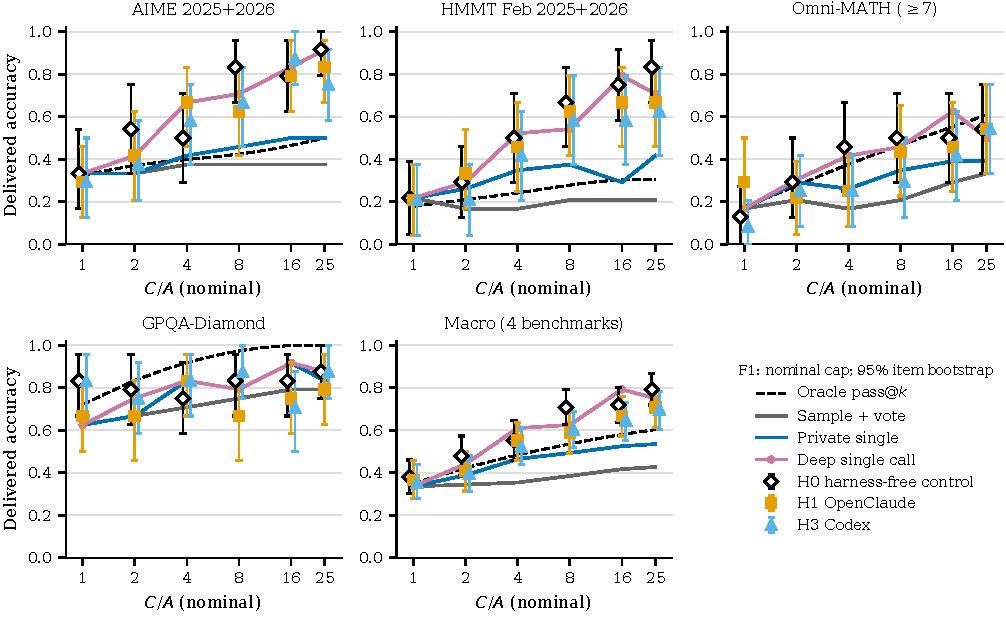
\includegraphics[width=\textwidth]{figures/d2_ladder_f1.pdf}
\caption{The ladder curves with the harness cells at nominal $C$ (F1). Error bars: 95\% paired item bootstrap.}
\label{fig:f1}
\end{figure}

\subsection{Primary family}

Anchor first: H0/16 $-$ deep/16 = $-$7.3 points
[$-$15.5, $-$0.3] on the same host in the same week, which
is the part of any harness shortfall that is not orchestration. Table~\ref{tab:primary} gives the four
pre-registered contrasts with Holm-adjusted $p$-values over exactly four.

\begin{table}[htbp]
\centering\small
\adjustbox{max width=\textwidth}{\begin{tabular}{lrrrrl}
\toprule
Contrast (macro, 96 items) & estimate (pts) & 95\% CI (pts) & $p$ & Holm $p$ & reading \\ \midrule
\texttt{H0/16-deep/16} & $-$7.3 & [$-$15.5, $-$0.3] & -- & -- & loses to fixed rule \\
\texttt{H1/16-deep/16} & $-$12.5 & [$-$21.3, $-$5.2] & 0.004 & 0.004 & loses to fixed rule \\
\texttt{H1/16-sample/16} & +25.0 & [+15.1, +34.7] & 0.000 & 0.000 & above baseline \\
\texttt{H3/16-deep/16} & $-$14.6 & [$-$23.4, $-$7.1] & 0.001 & 0.003 & loses to fixed rule \\
\texttt{H3/16-sample/16} & +22.9 & [+13.1, +33.2] & 0.000 & 0.000 & above baseline \\
\bottomrule
\end{tabular}
}
\caption{Anchor and the primary family (96 items, macro; studentized item-cluster bootstrap; Holm
over four). Reading rule, frozen before collection: CI below 0 against deep/16 means dynamic orchestration loses
to the fixed rule at $16A$; CI containing 0 is inconclusive at $n$ = 96; CI above 0 means the rule is
incomplete.}
\label{tab:primary}
\end{table}

\begin{figure}[htbp]
\centering
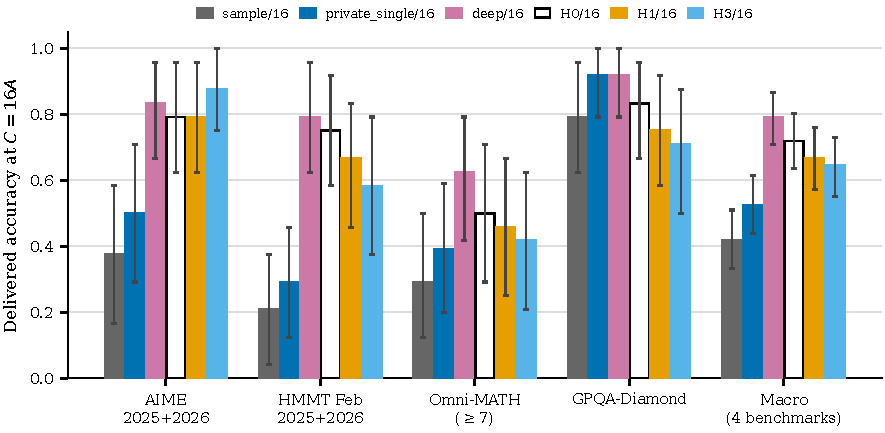
\includegraphics[width=\textwidth]{figures/d5_per_benchmark.pdf}
\caption{Per benchmark at $C = 16A$ ($n$ = 24 each, descriptive).}
\label{fig:bench}
\end{figure}

\subsection{Descriptive set, realized frontier and dollars}

Slope per doubling of $C$ (macro points): H1 +7.6, H3 +7.7, H0 +8.9, against
the ladder's deep +9.6, revision +4.4 and vote +2.1.
Against the paired per-item oracle pass@16, H1/16 is +8.8 points
[$-$1.7, +19.2] and H3/16
+7.7 points. The full arm $\times$ rung set, with every comparator, is in
\texttt{tables/rung\_table.csv} and \texttt{tables/descriptive.csv}.

\begin{figure}[htbp]
\centering
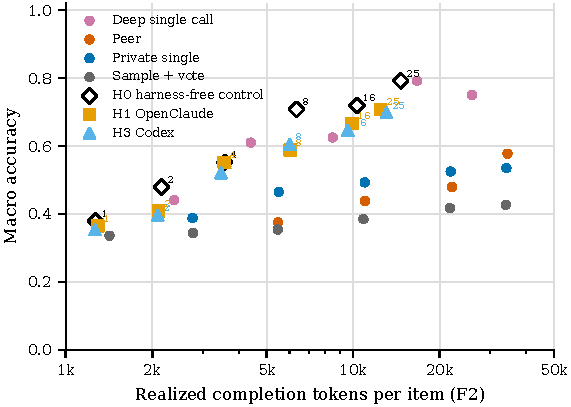
\includegraphics[width=0.48\textwidth]{figures/d3_realized_f2.pdf}\hfill
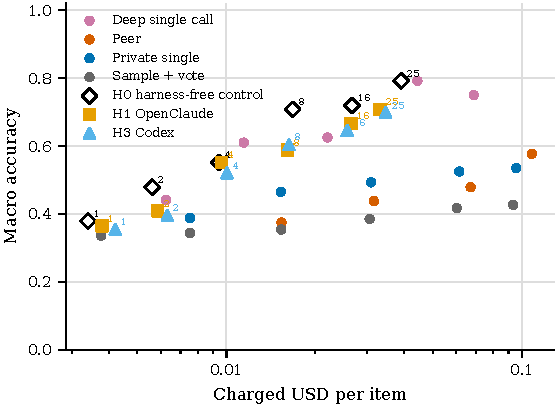
\includegraphics[width=0.48\textwidth]{figures/d4_dollars.pdf}
\caption{Left: F2, both sides at realized completion tokens per item. Right: charged USD per item. Descriptive
frontiers among evaluated configurations.}
\label{fig:frontiers}
\end{figure}

\begin{table}[htbp]
\centering\small
\adjustbox{max width=\textwidth}{\begin{tabular}{lrrrrr}
\toprule
configuration & nominal $C$ & realized completion & prompt tokens & USD (charged) & macro accuracy \\ \midrule
\texttt{H0/1} & 1,024 & 1,269 & 1,913 & 0.0034 & 0.379 \\
\texttt{H1/1} & 1,024 & 1,294 & 3,987 & 0.0038 & 0.365 \\
\texttt{H3/1} & 1,024 & 1,263 & 6,254 & 0.0042 & 0.354 \\
\texttt{H0/2} & 2,048 & 2,152 & 2,639 & 0.0056 & 0.479 \\
\texttt{H1/2} & 2,048 & 2,100 & 4,558 & 0.0059 & 0.409 \\
\texttt{H3/2} & 2,048 & 2,090 & 6,740 & 0.0063 & 0.396 \\
\texttt{H0/4} & 4,096 & 3,568 & 3,726 & 0.0095 & 0.552 \\
\texttt{H1/4} & 4,096 & 3,558 & 5,650 & 0.0096 & 0.552 \\
\texttt{H3/4} & 4,096 & 3,470 & 7,948 & 0.0100 & 0.521 \\
\texttt{H0/8} & 8,192 & 6,352 & 5,999 & 0.0168 & 0.708 \\
\texttt{H1/8} & 8,192 & 6,040 & 7,089 & 0.0161 & 0.588 \\
\texttt{H3/8} & 8,192 & 6,021 & 9,471 & 0.0163 & 0.604 \\
\texttt{H0/16} & 16,384 & 10,330 & 7,409 & 0.0266 & 0.719 \\
\texttt{H1/16} & 16,384 & 9,904 & 8,380 & 0.0265 & 0.667 \\
\texttt{H3/16} & 16,384 & 9,585 & 10,702 & 0.0256 & 0.646 \\
\texttt{H0/25} & 25,600 & 14,638 & 8,705 & 0.0390 & 0.792 \\
\texttt{H1/25} & 25,600 & 12,472 & 9,632 & 0.0331 & 0.708 \\
\texttt{H3/25} & 25,600 & 13,060 & 12,966 & 0.0346 & 0.698 \\
\texttt{deep/1} & 1,024 & 1,420 & 1,908 & 0.0038 & 0.336 \\
\texttt{private\_single/1} & 1,024 & 1,420 & 1,908 & 0.0038 & 0.336 \\
\texttt{sample/1} & 1,024 & 1,420 & 1,908 & 0.0038 & 0.336 \\
\texttt{deep/2} & 2,048 & 2,386 & 2,932 & 0.0062 & 0.441 \\
\texttt{peer/2/0} & 2,048 & 2,769 & 3,815 & 0.0075 & 0.344 \\
\texttt{peer/2/1} & 2,048 & 5,480 & 10,729 & 0.0154 & 0.375 \\
\texttt{peer/2/3} & 2,048 & 10,989 & 24,258 & 0.0316 & 0.438 \\
\texttt{private\_single/2} & 2,048 & 2,761 & 4,686 & 0.0075 & 0.388 \\
\texttt{sample/2} & 2,048 & 2,769 & 3,815 & 0.0075 & 0.344 \\
\texttt{deep/4} & 4,096 & 4,403 & 4,980 & 0.0115 & 0.610 \\
\texttt{peer/4/3} & 4,096 & 22,084 & 66,386 & 0.0670 & 0.479 \\
\texttt{private\_single/4} & 4,096 & 5,507 & 10,021 & 0.0153 & 0.465 \\
\texttt{sample/4} & 4,096 & 5,463 & 7,630 & 0.0154 & 0.354 \\
\texttt{peer/5/4} & 5,120 & 34,455 & 121,374 & 0.1080 & 0.577 \\
\texttt{deep/8} & 8,192 & 8,498 & 9,075 & 0.0220 & 0.625 \\
\texttt{private\_single/8} & 8,192 & 10,968 & 20,749 & 0.0309 & 0.493 \\
\texttt{sample/8} & 8,192 & 10,864 & 15,260 & 0.0305 & 0.385 \\
\texttt{deep/16} & 16,384 & 16,686 & 17,267 & 0.0443 & 0.792 \\
\texttt{private\_single/16} & 16,384 & 21,841 & 42,102 & 0.0613 & 0.525 \\
\texttt{sample/16} & 16,384 & 21,722 & 30,521 & 0.0602 & 0.417 \\
\texttt{deep/25} & 25,600 & 25,894 & 26,483 & 0.0687 & 0.750 \\
\texttt{private\_single/25} & 25,600 & 34,155 & 66,282 & 0.0957 & 0.535 \\
\texttt{sample/25} & 25,600 & 33,985 & 47,689 & 0.0934 & 0.427 \\
\bottomrule
\end{tabular}
}
\caption{Realized tokens and dollars per item for the comparators and the harness cells.}
\label{tab:cost}
\end{table}

\subsection{Realized budget and harness diagnostics}

\begin{table}[htbp]
\centering\small
\adjustbox{max width=\textwidth}{\begin{tabular}{lrrrrrrr}
\toprule
cell & $C$ & mean & median & realized share & grace & cap-bound & terminal \\ \midrule
\texttt{H0/1} & 1,024 & 981 & 1,024 & 0.958 & 290 & 0.885 & 0.000 \\
\texttt{H0/2} & 2,048 & 1,864 & 2,048 & 0.910 & 288 & 0.812 & 0.000 \\
\texttt{H0/4} & 4,096 & 3,336 & 4,096 & 0.814 & 232 & 0.688 & 0.000 \\
\texttt{H0/8} & 8,192 & 6,124 & 8,192 & 0.748 & 228 & 0.625 & 0.000 \\
\texttt{H0/16} & 16,384 & 10,180 & 11,232 & 0.621 & 150 & 0.406 & 0.000 \\
\texttt{H0/25} & 25,600 & 14,525 & 14,209 & 0.567 & 113 & 0.312 & 0.000 \\
\texttt{H1/1} & 1,024 & 963 & 1,024 & 0.941 & 331 & 0.865 & 0.000 \\
\texttt{H1/2} & 2,048 & 1,794 & 2,048 & 0.876 & 312 & 0.750 & 0.000 \\
\texttt{H1/4} & 4,096 & 3,301 & 4,096 & 0.806 & 257 & 0.656 & 0.000 \\
\texttt{H1/8} & 8,192 & 5,794 & 8,192 & 0.707 & 272 & 0.521 & 0.000 \\
\texttt{H1/16} & 16,384 & 9,730 & 10,733 & 0.594 & 174 & 0.344 & 0.000 \\
\texttt{H1/25} & 25,600 & 12,346 & 10,760 & 0.482 & 126 & 0.271 & 0.000 \\
\texttt{H3/1} & 1,024 & 961 & 1,024 & 0.938 & 302 & 0.865 & 0.000 \\
\texttt{H3/2} & 2,048 & 1,797 & 2,048 & 0.877 & 294 & 0.750 & 0.000 \\
\texttt{H3/4} & 4,096 & 3,212 & 4,096 & 0.784 & 258 & 0.677 & 0.000 \\
\texttt{H3/8} & 8,192 & 5,807 & 8,192 & 0.709 & 214 & 0.542 & 0.000 \\
\texttt{H3/16} & 16,384 & 9,441 & 10,189 & 0.576 & 144 & 0.344 & 0.000 \\
\texttt{H3/25} & 25,600 & 12,934 & 11,094 & 0.505 & 126 & 0.292 & 0.000 \\
\bottomrule
\end{tabular}
}
\caption{Nominal cap beside realized completion (mean, median), realized share, mean grace, share of runs with a
cap-bound call and share closed by the terminal answer.}
\label{tab:realized}
\end{table}

\begin{table}[htbp]
\centering\small
\adjustbox{max width=\textwidth}{\begin{tabular}{lrrrrrrrrr}
\toprule
cell & calls & root & solver & spawns & spawn share & orch.\ share & abstain & parse fail & wall s \\ \midrule
\texttt{H0/1} & 1.0 & 1.0 & 0.0 & 0.00 & 0.000 & 1.000 & 0.010 & 0.000 & 19 \\
\texttt{H0/2} & 1.0 & 1.0 & 0.0 & 0.00 & 0.000 & 1.000 & 0.000 & 0.000 & 34 \\
\texttt{H0/4} & 1.0 & 1.0 & 0.0 & 0.00 & 0.000 & 1.000 & 0.000 & 0.000 & 56 \\
\texttt{H0/8} & 1.0 & 1.0 & 0.0 & 0.00 & 0.000 & 1.000 & 0.000 & 0.000 & 95 \\
\texttt{H0/16} & 1.0 & 1.0 & 0.0 & 0.00 & 0.000 & 1.000 & 0.000 & 0.000 & 150 \\
\texttt{H0/25} & 1.0 & 1.0 & 0.0 & 0.00 & 0.000 & 1.000 & 0.000 & 0.000 & 217 \\
\texttt{H1/1} & 1.0 & 1.0 & 0.0 & 0.00 & 0.000 & 1.000 & 0.052 & 0.000 & 21 \\
\texttt{H1/2} & 1.0 & 1.0 & 0.0 & 0.00 & 0.000 & 1.000 & 0.062 & 0.000 & 34 \\
\texttt{H1/4} & 1.0 & 1.0 & 0.0 & 0.00 & 0.000 & 1.000 & 0.021 & 0.000 & 53 \\
\texttt{H1/8} & 1.0 & 1.0 & 0.0 & 0.00 & 0.000 & 1.000 & 0.062 & 0.000 & 88 \\
\texttt{H1/16} & 1.0 & 1.0 & 0.0 & 0.00 & 0.000 & 1.000 & 0.042 & 0.000 & 140 \\
\texttt{H1/25} & 1.0 & 1.0 & 0.0 & 0.00 & 0.000 & 1.000 & 0.031 & 0.000 & 170 \\
\texttt{H3/1} & 1.0 & 1.0 & 0.0 & 0.00 & 0.000 & 1.000 & 0.062 & 0.000 & 20 \\
\texttt{H3/2} & 1.0 & 1.0 & 0.0 & 0.00 & 0.000 & 1.000 & 0.094 & 0.000 & 33 \\
\texttt{H3/4} & 1.0 & 1.0 & 0.0 & 0.00 & 0.000 & 1.000 & 0.000 & 0.000 & 52 \\
\texttt{H3/8} & 1.0 & 1.0 & 0.0 & 0.00 & 0.000 & 1.000 & 0.031 & 0.000 & 88 \\
\texttt{H3/16} & 1.0 & 1.0 & 0.0 & 0.00 & 0.000 & 1.000 & 0.000 & 0.000 & 133 \\
\texttt{H3/25} & 1.1 & 1.1 & 0.0 & 0.00 & 0.000 & 1.000 & 0.021 & 0.000 & 185 \\
\bottomrule
\end{tabular}
}
\caption{Harness diagnostics per cell: calls by conversation class, spawns, orchestrator token share, abstention
(no valid \texttt{<final>}), tool-call parse failures and wall time.}
\label{tab:diag}
\end{table}

\begin{figure}[htbp]
\centering
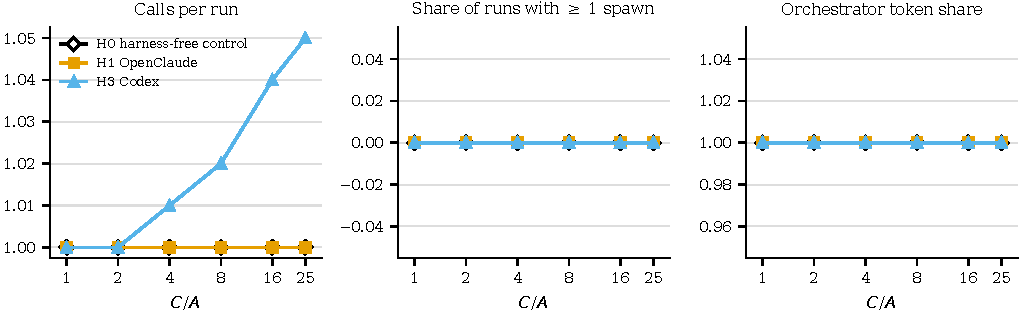
\includegraphics[width=\textwidth]{figures/d6_diagnostics.pdf}
\caption{Calls per run, spawn share and orchestrator token share against $C/A$.}
\label{fig:diag}
\end{figure}

\begin{figure}[htbp]
\centering
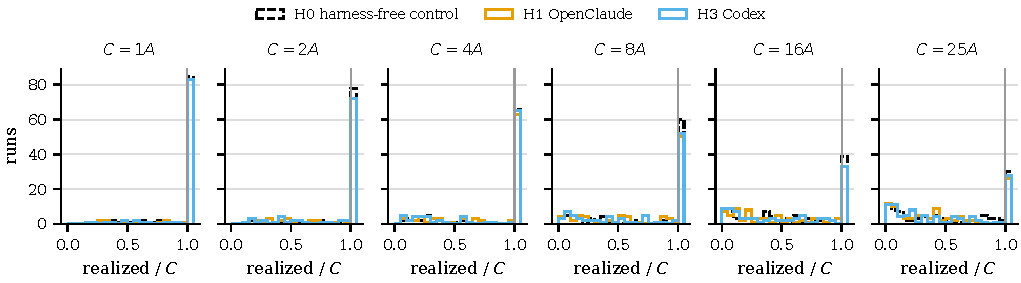
\includegraphics[width=\textwidth]{figures/d7_cap_binding.pdf}
\caption{Realized share of the cap per run, by rung and arm.}
\label{fig:cap}
\end{figure}

Scaffolding: the first root call of H1 carries 1,492 more prompt tokens than the H0
call on the same item and rung (SD 5,154, $n$ = 576);
H3 3,628 (SD 5,540). Spend: \$27.42 on the
current attempts, \$28.13 over every attempt (16 reruns).

\subsection{Provider sensitivity}

58 of the ladder's items were generated on Mancer and
38 on Parasail; 100.0\% of the harness cells ran on the
same provider as their ladder rows (96 items).

\begin{table}[htbp]
\centering\small
\adjustbox{max width=\textwidth}{\begin{tabular}{lrrr}
\toprule
contrast & Mancer items & Parasail items & same provider only \\ \midrule
\texttt{H0/16-deep/16} & $-$6.9 [$-$17.0, +1.9] ($n$=58) & $-$8.3 [$-$19.2, +2.2] ($n$=38) & $-$7.3 [$-$14.6, +0.0] ($n$=96) \\
\texttt{H1/16-deep/16} & $-$15.4 [$-$27.4, $-$4.8] ($n$=58) & $-$8.1 [$-$18.3, +0.0] ($n$=38) & $-$12.5 [$-$20.8, $-$5.2] ($n$=96) \\
\texttt{H1/16-sample/16} & +24.9 [+13.0, +36.9] ($n$=58) & +25.6 [+10.0, +41.1] ($n$=38) & +25.0 [+15.6, +34.4] ($n$=96) \\
\texttt{H3/16-deep/16} & $-$11.9 [$-$22.1, $-$1.7] ($n$=58) & $-$18.9 [$-$32.2, $-$8.1] ($n$=38) & $-$14.6 [$-$22.9, $-$7.3] ($n$=96) \\
\texttt{H3/16-sample/16} & +28.3 [+16.4, +40.4] ($n$=58) & +14.7 [$-$0.6, +30.0] ($n$=38) & +22.9 [+13.5, +32.3] ($n$=96) \\
\bottomrule
\end{tabular}
}
\caption{Every primary contrast restricted to the Mancer items, the Parasail items, and the items whose harness
run and ladder rows share a provider.}
\label{tab:provider}
\end{table}

\begin{figure}[htbp]
\centering
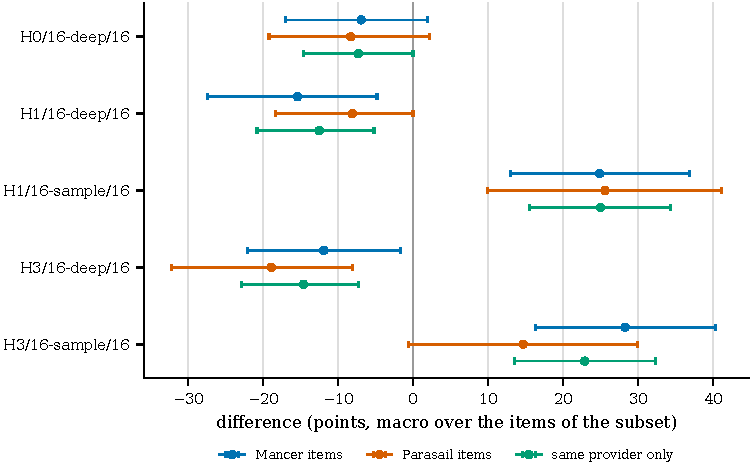
\includegraphics[width=0.8\textwidth]{figures/d8_provider_sensitivity.pdf}
\caption{Provider-stratified estimates of the anchor and the primary family.}
\label{fig:provider}
\end{figure}

\subsection{Repeat agreement}

Second-repeat cells available: 0 (extension E1; \texttt{tables/repeat\_agreement.csv}).

\begin{figure}[htbp]
\centering
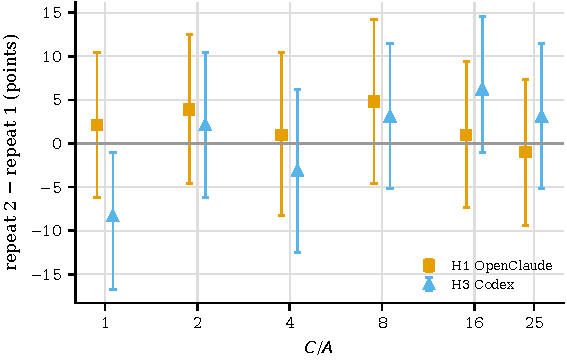
\includegraphics[width=0.6\textwidth]{figures/d9_repeat_agreement.pdf}
\caption{Repeat 2 minus repeat 1 per cell with the empirical run-to-run interval, when E1 ran.}
\label{fig:repeat}
\end{figure}

\section{Interpretation}
\label{sec:interp}

\paragraph{The orchestrators did not orchestrate.} Across all 1,728 main runs,
0 spawned a sub-agent, at any budget. OpenClaude made exactly one model call in each of
its 576 runs. Codex made one call in 564 runs and a
second in 12 (2.1\%). In every one of those, the
first call had invoked \texttt{update\_plan}, Codex's planning tool, and the second call
wrote the answer; none delegated. Both harnesses exposed delegation tools (\texttt{Agent} in
OpenClaude; \texttt{spawn\_agent} and its companions in Codex), and the task prompt stated the budget.
The model spent the budget thinking in one call. Behaviourally, the ``dynamic orchestrator'' in this study is one
natural-length call inside the harness's scaffolding.

\paragraph{At the nominal budget the fixed rule wins.} H1/16 $-$ deep/16 = $-$12.5
points [$-$21.3, $-$5.2], $p_{\text{Holm}}
= 0.004$; H3/16 $-$ deep/16 = $-$14.6 points
[$-$23.4, $-$7.1], $p_{\text{Holm}}
= 0.003$. The anchor splits each gap into two parts (Table~\ref{tab:decomp}).
H0/16 $-$ deep/16 = $-$7.3 points [$-$15.5,
$-$0.3] is the cost of a natural stop against a forced, exact spend; it is common to
both harnesses. H/16 $-$ H0/16 is the scaffolding part: $-$5.2 points
[$-$14.0, +3.1] for H1 and
$-$7.3 points [$-$16.4,
+1.2] for H3. The harness adds about 1.5k (H1)
and 3.6k (H3) prompt tokens of tool schemas and wrappers that no run used, and
the point estimates say this costs accuracy. Both intervals include zero, so at 96 items the size of
the scaffolding cost is not pinned down. The decomposition is descriptive, with no $p$-values: it was not in the
primary family.

\begin{table}[htbp]
\centering\small
\begin{tabular}{lrrrr}
\toprule
 & total & natural stop & scaffolding & prompt tokens \\
harness & H/16 $-$ deep/16 & H0/16 $-$ deep/16 & H/16 $-$ H0/16 & added \\
\midrule
H1 & $-$12.5 [$-$21.3, $-$5.2]
   & $-$7.3 [$-$15.5, $-$0.3]
   & $-$5.2 [$-$14.0, +3.1]
   & 1,492 \\
H3 & $-$14.6 [$-$23.4, $-$7.1]
   & $-$7.3 [$-$15.5, $-$0.3]
   & $-$7.3 [$-$16.4, +1.2]
   & 3,628 \\
\bottomrule
\end{tabular}
\caption{The gap to deep/16 at $C = 16A$ split by the anchor (macro points, 95\% studentized item-cluster
bootstrap CIs, 96 paired items). The two parts add up to the total. The first column is the primary
contrast; the scaffolding column is descriptive. Prompt tokens added: the first root call's prompt minus the H0
call's prompt on the same item and rung, mean over all rungs.}
\label{tab:decomp}
\end{table}

\paragraph{Why the natural call loses at nominal $C$: it stops early.} At $16A$ the mean realized share of the cap
is 0.59 for H1, 0.58 for H3 and
0.62 for H0 (Table~\ref{tab:realized}); only 34.4\% of
H1/16 runs and 34.4\% of H3/16 runs reached the cap. The ladder forced deep/16 to spend
exactly 16,384 reasoning tokens. Per realized token (F2, Figure~\ref{fig:frontiers}, left), the harness
points lie on or near the deep-call curve. Table~\ref{tab:rvd} makes this exact: each cell against the deep-call
accuracy interpolated at the same realized completion tokens. For the 10 harness
cells the difference runs from $-$4.1 to +0.4
points (mean $-$1.2 for H1, $-$1.7 for
H3), and 0 of the 10 intervals exclude zero. H0 sits above the curve
in all 5 cells, by +0.7 to
+8.3 points; the interval excludes zero at
\texttt{H0/8}.

The implication is narrow. The rule's advantage at the nominal budget comes from making the model spend its whole
budget. The ladder did that by forcing decoding, and no off-the-shelf harness offers it. It is not evidence that
orchestration decisions are worse: no orchestration decision was made.

\begin{table}[htbp]
\centering\small
\adjustbox{max width=\textwidth}{\begin{tabular}{lrrrr}
\toprule
cell & realized tokens & accuracy & deep at same tokens & difference (pts) [95\% CI] \\ \midrule
\texttt{H0/2} & 2,152 & 0.479 & 0.420 & +6.3 [$-$1.1, +13.8] \\
\texttt{H0/4} & 3,568 & 0.552 & 0.552 & +0.7 [$-$6.5, +8.0] \\
\texttt{H0/8} & 6,352 & 0.708 & 0.618 & +8.3 [+2.2, +15.0] \\
\texttt{H0/16} & 10,330 & 0.719 & 0.673 & +4.6 [$-$3.5, +12.6] \\
\texttt{H0/25} & 14,638 & 0.792 & 0.760 & +3.2 [$-$2.8, +9.4] \\
\texttt{H1/2} & 2,100 & 0.409 & 0.415 & $-$0.6 [$-$9.1, +8.0] \\
\texttt{H1/4} & 3,558 & 0.552 & 0.551 & $-$0.6 [$-$9.1, +8.1] \\
\texttt{H1/8} & 6,040 & 0.588 & 0.617 & $-$4.1 [$-$11.9, +3.5] \\
\texttt{H1/16} & 9,904 & 0.667 & 0.663 & +0.4 [$-$7.3, +7.5] \\
\texttt{H1/25} & 12,472 & 0.708 & 0.720 & $-$1.1 [$-$8.1, +5.0] \\
\texttt{H3/2} & 2,090 & 0.396 & 0.414 & $-$1.6 [$-$8.4, +5.0] \\
\texttt{H3/4} & 3,470 & 0.521 & 0.544 & $-$2.0 [$-$10.1, +6.3] \\
\texttt{H3/8} & 6,021 & 0.604 & 0.617 & $-$0.9 [$-$8.3, +6.3] \\
\texttt{H3/16} & 9,585 & 0.646 & 0.655 & $-$0.9 [$-$9.5, +7.4] \\
\texttt{H3/25} & 13,060 & 0.698 & 0.731 & $-$3.3 [$-$11.6, +4.0] \\
\bottomrule
\end{tabular}
}
\caption{Each cell against the deep call at the same realized completion tokens per item (F2, macro,
descriptive). The deep accuracy is interpolated log-linearly in realized tokens between the two adjacent deep
rungs. The difference and its 95\% CI are one paired linear contrast (cell minus the weighted pair of deep
columns) over the items known in all three columns, so it can differ by a point from the difference of the two
printed accuracies. The rung-1 cells realized fewer tokens than deep/1
(1,420) and are left out.}
\label{tab:rvd}
\end{table}

\paragraph{Against the naive baseline and the oracle.} Both harnesses beat sample/16 with vote by a wide
margin: H1/16 $-$ sample/16 = +25.0 points
[+15.1, +34.7], $p_{\text{Holm}}
< 0.001$; H3/16 $-$ sample/16 = +22.9 points
[+13.1, +33.2], $p_{\text{Holm}}
< 0.001$. Both also exceed the paired per-item oracle pass@16
(0.580): H1/16 by +8.8 points
[$-$1.7, +19.2] and H3/16 by
+7.7 points [$-$2.1,
+17.2]. Those two intervals include zero. In point estimate, one unforced call at $16A$ does better than a
perfect selector over the samples of sample/16 would.

\paragraph{Scope.} One model (Qwen3.8-27B); 96 items on 4 hard math and
science benchmarks; orchestration-only tools (no code execution, no search); one realisation per cell.
Orchestration itself was not exercised, so this does not show that orchestration is useless. It shows that these
two harnesses, as shipped, did not choose to orchestrate this model on these tasks. E0, in which the root's own
calls are capped at \texttt{max(A, C/4)}, is running; its results will be added.

\section{What to do with this}

For this model on these tasks, spend the budget on one deep call and force it to use the whole budget; neither
harness adds anything over that, and each adds unused prompt overhead. If a harness is used for other reasons,
expect it to behave like one unforced call that stops at about 0.59 of the cap. The
rule would change with a harness that actually delegates, with tools that add information a single call cannot
produce (code execution, search), or with a model that spends a long budget without being forced.

\section{Cost re-fit}

Re-fitted from the measured runs (Parasail prices, 25.0\% contingency), the core would cost
\$26.12; per-cell figures are in \texttt{tables/forecast\_refit.csv}.

\appendix
\section{Run facts and deviations}
\label{app:facts}

\paragraph{Spend.} The current attempts of the core cost \$27.42. The ledger charges every main attempt together
\$28.13: \$27.44 settled by the provider plus
\$0.69 charged at the full reservation for the
16 calls the provider cut mid-stream, which the provider billed at close to
nothing (contract \S10.39). The 16 attempts that reruns replaced cost \$0.72. The canary cost
\$0.50 over both executions (the superseded first one
\$0.25), and the pilot \$2.65. The study total,
canary and pilot included and E0 excluded, is \$30.59 settled, at most
\$31.28 with the conservative charges. The OpenRouter key agreed with the ledger at every
gate.

\paragraph{Gates.} Gate~1 (canary) and Gate~2 (pilot) advanced with owner-waived delegation criteria (contract
\S10.37). The canary's $16A$ probe had 0 of 4
runs spawning, which trips the pre-registered stop-and-ask. At Gate~2, 0 of
32 H1 runs and 0 of 32
H3 runs at $16A$ spawned. The owner's decision, recorded in
\texttt{run\_decisions.jsonl}: ``Run the core as planned'', because ``non-delegation is the finding; waive the pilot's delegation threshold and the live Codex tool-loop check (verified offline at Gate 0); the capped variant stays first in line after the core''.
The waived criteria stay recorded as failed, and nothing else was waivable: money, accounting, grants, provider
pinning, answers and forecast criteria stayed binding. The final Gate~4 passed every criterion.

\paragraph{Defects found and fixed during the run.}
\begin{itemize}
\item \textbf{The grace offered tools (\S10.28).} In the first canary the answer continuation after a cap-bound
call still carried the tool schemas, so some harness runs spent their one grace on a tool call and had no budget left
to answer. Every spawn recorded anywhere in the study (1 in all) was issued inside
such a grace. The grace now carries no tools, as the plan said; the 10 canary cells were
superseded and re-run (\S10.35).
\item \textbf{The upstream-failure latch (\S10.38).} The provider cut 16 main-stage
calls mid-stream (12 error envelopes, 4
ambiguous timeouts). H0 recorded these as transport failures and re-ran them
(8 reruns). Both harnesses instead retried the failed call into the proxy's
no-thinking terminal answer, which was scored as a model outcome. The first upstream failure now ends the run as an
infrastructure rerun, and the 8 main cells completed under the defect
(5 H1, 3 H3) were
invalidated and re-executed.
\item \textbf{Reconciliation rules (\S10.36, \S10.39, \S10.41).} The key's usage lags the ledger, so the dollar
check now waits for it to converge; it compares the key with the ledger's bounds (settled, settled plus
conservative charges) rather than the upper figure; and a failed call charged at its full grant is checked as an
upper bound. No recorded dollar changed.
\item \textbf{Gate~4's grader re-run (\S10.40).} The first Gate~4 counted
26 mismatches, all the same \texttt{INVALID\_OUTPUT} verdict both times: a
well-formed final answer the grader cannot parse, scored 0. The check compared the raw verdict instead of the
scored value. It now uses the scoring rule; stored scores were already right and did not change.
\end{itemize}

\paragraph{The first main launch.} It was submitted without the account auto-reload flag, so its active ceiling
was \$49.84 instead of the approved \$95.00.
It was drained after 5.3 minutes and resubmitted with the flag; its
50 finished cells were kept.

None of these changed a pre-registered scientific rule. Each made the code match the plan or fixed a check.

\end{document}
